\chapter{Perturbing the lattice}

In this chapter we will derive an effective spin Hamiltonian for different models in the presence of a high frequency electromagnetic perturbation. The goal is to manipulate $J$ and $\bs{D}_{ij}$ in \ref{HeffNOEMF} separately. This has already been done for the case of Mott insulators (\cite{Mentink2015}, \cite{Kitamura2017}) where the starting Hamiltonian is the Hubbard model:

\begin{equation*}
\hat{H} = -t_0\sum_{\langle i,j \rangle, \sigma} \hat{c}_{i \sigma}^\dagger \hat{c}_{j \sigma} + \text{U} \sum_{i=1}^M \hat{n}_{i\uparrow}\hat{n}_{i\downarrow}
\end{equation*} 

In this model, since SOI is not taken into account, only the exchange interaction $J$ plays a role. The electromagnetic perturbation is then introduced via the Peierls substitution. We reproduce the result in section \ref{Section3Hubbard}. In the following sections we extend the analysis to different systems with spin orbit interaction thereby modulating $\bs{D}_{ij}$ or other spin interactions. The simplest model with spin orbit interaction is \ref{Hubbard}:

\begin{equation*}
\hat{H} = -\sum_{\langle i,j \rangle, \sigma, \sigma'}(\delta_{\sigma, \sigma'} t_{0} + \bs{\Delta}_{ij} \bs{\sigma}_{\sigma, \sigma'})\hat{c}_{i \sigma}^\dagger \hat{c}_{j \sigma'} + \text{U} \sum_{i=1}^M \hat{n}_{i\uparrow}\hat{n}_{i\downarrow}
\end{equation*}

Which is the same Hubbard model plus a spin dependent hopping term, which represents Rashba SOI for $\bs{\Delta}_{ij} = i\Delta_R(R_{ij}^y, -R_{ij}^x, 0)$ or Dresselhaus SOI for $\bs{\Delta}_{ij} = i\Delta_R(R_{ij}^x, -R_{ij}^y, 0)$. In section \ref{Section3HubbardSOI} we show how the exchange interaction and the DMI couplings are modulated in presence of an electromagnetic field.  

In the case of graphene or other coplanar honeycomb lattice structures, nearest neighbor Rashba terms are not allowed by symmetry, and only next nearest neighbor (NNN) spin conserving terms contribute \cite{Kane2005}, this term opens a gap in the band structure describing a topological insulator. For this case we examine the Kane-Mele-Hubbard model. The effective spin model of this Hamiltonian contains the usual exchange interaction and DMI and, in addition, it exhibits anisotropic exchange interaction arising from the intrinsic SOI term. This new term has already been obtained in \cite{Rachel2010} without taking into account any electromagnetic field.

Non-coplanar honeycomb lattice may exhibit intrinsic Rashba interactions between NNN \cite{Liu2011}, this, together with a NNN hopping (which would arise from direct overlapping of the next nearest neighbor Wannier functions or from second order processes) will lead to NNN DMI.


\begin{section}{Time dependent effective Hamiltonian}
\label{SectionTDHeff}

In this section we will derive a general effective Hamiltonian starting with any Hamiltonian that can be written as:

\begin{equation}
\hat{H} = -\hat{T} + \text{U}\hat{D}
\end{equation}
Where $\hat{D} = \sum_{i=1}^M \hat{n}_{i\uparrow}\hat{n}_{i\downarrow}$ is the doublon number operator and $\hat{T}$ is any hopping operator. In terms of on-site creation and annihilation operators we can write the hopping operator as $\hat{T} = \sum_{i,j, \sigma, \sigma'} t_{ij}^{\sigma \sigma'} \hat{c}_{i \sigma}^\dagger \hat{c}_{j \sigma'}$. The strength of the on-site interaction $\text{U}$ is much larger than the hopping amplitude, therefore, in a half filling system the zero double occupancies subspace $d=0$ can be taken as the low energy subspace in which the effective Hamiltonian will act.

The effect of the electromagnetic perturbation in the lattice can be introduced via the Peierls substitution (\ref{AP3A}). With this notation, in presence of a vector potential $\vec{A}(t)$ (which we assume to not vary noticeably in the scale of the lattice) the Peierls substitution leads to an extra time dependent phase in the hopping amplitude:

\begin{equation}
t_{ij}^{\sigma \sigma'}(t) = t_{ij}^{\sigma \sigma'} e^{ie\bs{R}_{ij}\cdot\bs{A}(t)}
\end{equation}
Where $\bs{A}$ is the vector potential and $\bs{R}_{ij} = \bs{R}_i-\bs{R}_j$. We write the electric field as $\bs{E}(t) = \frac{1}{2}(\vec{E}e^{-i\omega t}+\vec{E}^*e^{i\omega t})$, where $\vec{E} = E_0\hat{e}$ and $\hat{e} = \frac{1}{\sqrt{1+\lambda_{POL}^2}}(\hat{e}_x+i\lambda_{POL}\hat{e}_y)$ is the polarization vector and $\lambda_{POL} = 0, \pm 1$ for plane polarized, right handed and left handed circular polarized field respectively. The vector potential takes the form $\bs{A}(t) = \frac{1}{2}(\vec{A}e^{-i\omega t} + \vec{A}^* e^{i\omega t})$, with $\vec{A} = \frac{iE_0}{\omega}\hat{e}$.

Let us define:

\begin{equation}
\label{Def_alpha}
e\bs{R}_{ij}\vec{A} = \alpha_{ij} e^{i \theta_{ij}}
\end{equation}
With $\alpha_{ij} = \pm|e\bs{R}_{ij}\vec{A}|$ in such a way that:

\begin{align}
\alpha_{ij} &= -\alpha_{ji} \label{alphaSym} \\
\theta_{ij} &= \theta_{ji} \label{thetaSym}
\end{align}
and $\theta_{ij} \in \left[0,\pi\right)$. Then we can apply the Jacobi–Anger expansion:

\begin{align*}
t_{ij}^{\sigma \sigma'}(t) &= t_{ij}^{\sigma \sigma'}e^{ie\bs{R}_{ij}\cdot\bs{A}(t)} = t_{ij}^{\sigma \sigma'}e^{i\alpha_{ij} \cos(\omega t - \theta_{ij})} = \\
&= t_{ij}^{\sigma \sigma'}\sum_m e^{i(\frac{\pi}{2}-\theta_{ij})m} \mathcal{J}_m(\alpha_{ij}) e^{im\omega t} = \sum t_{ij,m}^{\sigma \sigma'} e^{im\omega t}
\end{align*}
Where we defined 

\begin{equation}
\label{HoppAmpFourier}
t_{ij,m}^{\sigma \sigma'} = t_{ij}^{\sigma \sigma'} e^{i(\frac{\pi}{2}-\theta_{ij})m} \mathcal{J}_m(\alpha_{ij})
\end{equation}
Which is the \textit{m}th Fourier mode of the hopping term and $\mathcal{J}_m(x)$ is the \textit{m}th Bessel function \cite{Kitamura2017}. Correspondingly we can write $\hat{T}(t) = \sum_m \hat{T}_m e^{im \omega t}$ where $\hat{T}_m$ is the sum of all the \textit{m}th Fourier mode of the hopping terms. We can further decompose the hopping operator into:

\begin{equation}
\hat{T}(t) = \sum_m (\hat{T}_{-1,m}+\hat{T}_{0,m}+\hat{T}_{1,m})e^{im\omega t}
\end{equation}
Where $\hat{T}_{dm}(t)$ changes the doublon number by $d$, for example, if $\hat{P}_d$ is the projection operator into the subspace with doublon number $d$, then $\hat{T}_{dm}(t) = \sum_i \hat{P}_{i+d}\hat{T}_{m}(t)\hat{P}_i$. Since the hopping term is of second order in the creation and annihilation operators, it can change the double occupancy of the states only by $\pm1$.

In order to derive the form of the effective spin Hamiltonian let us introduce a time dependent unitary transformation $\hat{U}(t) = e^{-i\hat{S}(t)}$. The transformed Hamiltonian is:

\begin{equation}
\hat{H}'(t) = e^{i\hat{S}(t)} \hat{H}(t) e^{-i\hat{S}(t)} - e^{i\hat{S}(t)} id_t e^{-i\hat{S}(t)}
\end{equation} 
We perform the unitary transformation perturbatively in the hopping operator, we can formally write $\hat{T}(t) = \eta \hat{T}(t)$, where $\eta$ will play the role of a bookkeeping parameter in the perturbative expansion. We expand $\hat{S}(t) = \sum_\nu \eta^\nu \hat{S}^{(\nu)}(t)$ and $\hat{H}'(t) = \sum_\nu \eta^\nu \hat{H}'^{(\nu)}(t)$. We require the transformed Hamiltonian to be block diagonal in the doublon number operator $\hat{d}$. To fulfill this requirement, the unitary transformation $\hat{S}(t)$ must have the same periodicity as $\hat{T}(t)$; consequently, the transformed Hamiltonian $\hat{H}'(t)$ will have the same periodicity as the original Hamiltonian $\hat{H}(t)$. Thus we can write $\hat{S}^{(\nu)}(t) = \sum_m e^{im\omega t}\hat{S}^{(\nu)}_m$. With the further requirement that $\hat{S}(t)$ does not contain block-diagonal terms, we can uniquely determine the unitary transformation:

\begin{equation}
\hat{S}^{(\nu)}(t) = \sum_{d \neq 0} \sum_m \eta^\nu \hat{S}^{(\nu)}_{d,m} e^{im\omega t}
\end{equation}
where $\hat{S}^{(\nu)}_{d,m}$ changes the double occupancy number by $d$.

Now we can use the identity:

\begin{equation}
id_t e^{-i\hat{S}(t)} = \sum_n \frac{1}{(n+1)!}\text{ad}_{-i\hat{S}(t)}^n (d_t \hat{S}(t))e^{-i\hat{S}(t)}
\end{equation}
Derived in appendix \ref{AP3B}, where $\text{ad}_A(B) = [A,B]$ to rewrite the transformed Hamiltonian as:

\begin{equation}
\hat{H}'(t) = e^{i\hat{S}(t)} \left( \hat{H}(t) - \sum_n \frac{1}{(n+1)!}\text{ad}_{-i\hat{S}(t)}^n (d_t \hat{S}(t)) \right) e^{-i\hat{S}(t)}
\end{equation}
Using the Baker–Campbell–Hausdorff expansion we can write the transformed Hamiltonian as:

\begin{equation}
\label{PertFull}
\hat{H}'(t) = \sum_m \frac{1}{m!} \text{ad}_{i\hat{S}(t)}^m \left( \hat{H}(t) - \sum_n \frac{1}{(n+1)!}\text{ad}_{-i\hat{S}(t)}^n (d_t \hat{S}(t)) \right)
\end{equation}
Now, in this expression we have to expand $\hat{S}(t) = \sum_\nu \eta^\nu \hat{S}^{(\nu)}(t)$ and $\hat{H}'(t) = \sum_\nu \eta^\nu \hat{H}'^{(\nu)}(t)$ and determine $\hat{S}^{(\nu)}(t)$ iteratively in $\nu$ so that $\hat{H}'^{(\nu)}(t)$ is diagonal in the doublon number. Notice that we do not expand $\hat{H}(t)$ as an infinite series since $\hat{H}(t) = -\eta \hat{T}(t) + \text{U}\hat{D}$. Now, notice also that if we take $i\hat{S}^{(0)}(t)=0$ in \ref{PertFull}, then, to zeroth order in $\eta$ only terms in $m=0$ and $n=0$ contribute obtaining:

\begin{equation}
\hat{H}'^{(0)}(t) = \text{U}\hat{D}
\end{equation}
Which is indeed diagonal in the doublon number, and therefore we can take $i\hat{S}^{(0)}(t)=0$. With this equating terms of the same order in \ref{PertFull} is greatly simplified, since terms with high $m,n$ will correspond to terms with high $\eta$. Since we are only interested in orders up to second order, we can truncate \ref{PertFull} up to $m=2$:

\begin{align}
\label{PertTrunc}
\hat{H}'(t) &=  \hat{H}(t) - \sum_n \frac{1}{(n+1)!}\text{ad}_{-i\hat{S}(t)}^n (d_t \hat{S}(t)) + [i\hat{S}(t), \hat{H}(t) - \sum_n \frac{1}{(n+1)!}\text{ad}_{-i\hat{S}(t)}^n (d_t \hat{S}(t))] + \nonumber \\
&+ \frac{1}{2} [i\hat{S}(t),[i\hat{S}(t), \hat{H}(t) - \sum_n \frac{1}{(n+1)!}\text{ad}_{-i\hat{S}(t)}^n (d_t \hat{S}(t)) ]]
\end{align}
This equation holds up to order $\eta^2$. In first order we obtain:

\begin{equation}
\label{1stO}
\hat{H}'^{(1)}(t) = -\hat{T}(t) - d_t\hat{S}^{(1)}(t) + \left[ i\hat{S}^{(1)}(t), \text{U}\hat{D} \right]
\end{equation}
Now we expanding in $m,d$ and use $\left[ \hat{D}, \hat{S}^{(\nu)}_{dm} \right] = d\hat{S}^{(\nu)}_{dm}$ because $\hat{S}^{(\nu)}_{dm}$ changes the doublon number by $d$:

\begin{equation}
\hat{H}'^{(1)}(t)=-\hat{T}(t)-\sum_{d\neq 0}\sum_m (\text{U}d+m\omega) i\hat{S}^{(1)}_{dm} e^{im\omega t}
\end{equation}
Therefore:

\begin{align}
i\hat{S}^{(1)}_d(t) &= -\sum_m \frac{\hat{T}_{d,m}}{\text{U}d+m\omega}e^{im\omega t} \label{1stOSpin}\\
\hat{H}'^{(1)}(t) &= -\sum_m \hat{T}_{0,m}(t)e^{im\omega t} \label{1stOH}
\end{align}
To second order we find:

\begin{align}
\hat{H}'^{(2)}(t) &= - d_t\hat{S}^{(2)}(t) - \frac{1}{2}\left[-i\hat{S}^{(1)}(t), d_t\hat{S}^{(1)}(t) \right] + \left[i\hat{S}^{(1)}(t), -\hat{T}(t)-\frac{1}{2}d_t\hat{S}^{(1)}(t) \right] +\nonumber \\
&+ \left[i\hat{S}^{(2)}(t), \text{U}\hat{D} \right] + \frac{1}{2} \left[i\hat{S}^{(1)}(t), \left[i\hat{S}^{(1)}(t), \text{U}\hat{D} \right] \right] = \nonumber \\
&= \left[i\hat{S}^{(2)}(t), \text{U} \hat{D} \right] - \left[ i\hat{S}^{(1)}(t), \hat{T}(t) \right] + \frac{1}{2}\left[ i\hat{S}^{(1)}(t), \left[ i\hat{S}^{(1)}(t), \text{U}\hat{D} \right] \right] - d_t\hat{S}^{(2)}(t)
\end{align}
Using \ref{1stO} and using $\left[ i\hat{S}^{(1)}(t), d_t\hat{S}^{(1)}(t)\right] = 0$ due to different Fourier modes of the hopping operator being equal up to a constant (explain better), we can rewrite:

\begin{equation}
\hat{H}'^{(2)}(t) = \left[i\hat{S}^{(2)}(t), \text{U} \hat{D} \right] - \frac{1}{2}\left[ i\hat{S}^{(1)}(t), \hat{T}(t) - \hat{H}'^{(1)}(t)\right] - d_t\hat{S}^{(2)}(t)
\end{equation}
Using \ref{1stOSpin} and \ref{1stOH}, the middle term is:

\begin{align*}
&\left[ i\hat{S}^{(1)}(t), \hat{T}(t) - \hat{H}'^{(1)}(t)\right] = -\left[\sum_m \left( \frac{\hat{T}_{1m}}{\text{U}+m\omega} - \frac{\hat{T}_{-1m}}{\text{U}-m\omega} \right)e^{im \omega t}, \sum_n \left( \hat{T}_{-1n} + 2\hat{T}_{0n} + \hat{T}_{1n} \right) e^{in\omega t} \right] \\
&= -\sum_{mn} \left\{ \frac{2\left[\hat{T}_{1m}, \hat{T}_{0n} \right]}{\text{U}+m\omega} + \frac{\left[\hat{T}_{1m}, \hat{T}_{-1n} \right]}{\text{U}+m\omega} - \frac{\left[\hat{T}_{-1m}, \hat{T}_{1n} \right]}{\text{U}-m\omega} - \frac{2\left[\hat{T}_{-1m}, \hat{T}_{0n} \right]}{\text{U}-m\omega} \right\} e^{i(m+n)\omega t} \\
&= -\sum_{mn} \left\{ \frac{2\left[\hat{T}_{1n}, \hat{T}_{0(m-n)} \right]}{\text{U}+n\omega} + \frac{\left[\hat{T}_{1n}, \hat{T}_{-1(m-n)} \right]}{\text{U}+n\omega} - \frac{\left[\hat{T}_{-1n}, \hat{T}_{1(m-n)} \right]}{\text{U}-n\omega} - \frac{2\left[\hat{T}_{-1n}, \hat{T}_{0(m-n)} \right]}{\text{U}-n\omega} \right\} e^{im\omega t}
\end{align*}
Altogether:

\begin{align*}
\hat{H}'^{(2)}(t) &= \sum_{mn} \left\{ \frac{\left[\hat{T}_{1n}, \hat{T}_{0(m-n)} \right]}{\text{U}+n\omega} + \frac{\left[\hat{T}_{1n}, \hat{T}_{-1(m-n)} \right]}{2(\text{U}+n\omega)} - \frac{\left[\hat{T}_{-1n}, \hat{T}_{1(m-n)} \right]}{2(\text{U}-n\omega)} - \frac{\left[\hat{T}_{-1n}, \hat{T}_{0(m-n)} \right]}{\text{U}-n\omega} \right\} e^{im\omega t} \\
&-\sum_{d\neq 0}\sum_m (\text{U}d+m\omega) i\hat{S}^{(2)}_{dm} e^{im\omega t}
\end{align*}
By choosing $i\hat{S}^{(2)}_{dm}$ such that the transformed Hamiltonian is block-diagonal, we obtain:

\begin{align}
i\hat{S}^{(2)}_{dm} &= \sum_n \frac{\left[ \hat{T}_{dn}, \hat{T}_{0(m-n)} \right]}{(\text{U}d+n\omega)(\text{U}d+m\omega)} \label{2ndOSpin}\\
\hat{H}'^{(2)}(t) &= \frac{1}{2}\sum_{mn} \left( \frac{\left[\hat{T}_{1n}, \hat{T}_{-1(m-n)} \right]}{\text{U}+n\omega} - \frac{\left[\hat{T}_{-1n}, \hat{T}_{1(m-n)} \right]}{\text{U}-n\omega} \right) e^{im\omega t} \label{2ndOH}
\end{align}
Now the effective Hamiltonian acts on the subspace of $d=0$ (zero double occupancies), therefore we are only interested on the block $\hat{P}_0 \hat{H}'^{(2)}(t) \hat{P}_0$ (notice that $\hat{P}_0 \hat{H}'^{(1)}(t) \hat{P}_0 = 0$). In this subspace we can write:

\begin{align}
\hat{H}_{\text{eff}}(t) &= \hat{P}_0\hat{H}'^{(2)}(t)\hat{P}_0 = -\frac{1}{2}\sum_{mn} \left( \frac{\hat{P}_0  \hat{T}_{-1(m-n)}\hat{T}_{1n}\hat{P}_0}{\text{U}+n\omega} + \frac{\hat{P}_0 \hat{T}_{-1n} \hat{T}_{1(m-n)} \hat{P}_0}{\text{U}-n\omega} \right) e^{im\omega t} \nonumber \\
&= -\frac{1}{2}\sum_{mn} \left\{ \frac{\hat{P}_0  (\hat{T}_{-1(m-n)}\hat{T}_{1n} + \hat{T}_{-1-n}\hat{T}_{1(m+n)})\hat{P}_0}{\text{U}+n\omega} \right\} e^{im\omega t} \label{2ndOHeff}
\end{align}
Now, since the hopping operators act on the subspace $d=0$ and must remain within that subspace, therefore $\hat{P}_0 \hat{T}_{-1a} \hat{T}_{1b} \hat{P}_0$ will be a sum of all possible hoppings between two different sites:

\begin{align*}
\hat{P}_0 \hat{T}_{-1a} \hat{T}_{1b} \hat{P}_0 = \sum_{i,j, \sigma_1, \sigma_2, \sigma_3, \sigma_4} t_{ij,a}^{\sigma_1 \sigma_2} t_{ji,b}^{\sigma_3 \sigma_4} \hat{c}_{i \sigma_1}^\dagger \hat{c}_{j \sigma_2} \hat{c}_{j \sigma_3}^\dagger \hat{c}_{i \sigma_4}
\end{align*}
Where $a$ and $b$ are any two Fourier modes. Inserting this into \ref{HeffSimplified} and using the definition of $t_{ij,m}^{\sigma \sigma'} = t_{ij}^{\sigma \sigma'} e^{i(\frac{\pi}{2}-\theta_{ij})m} \mathcal{J}_m(\alpha_{ij})$ and using that $\theta_{ji} = \theta_{ij}$ and $\alpha_{ji} = -\alpha_{ij}$ and the properties $\mathcal{J}_{-m}(x) = (-1)^m\mathcal{J}_m(x)$ and $\mathcal{J}_m(-x) = (-1)^m\mathcal{J}_m(x)$ we can write \ref{HeffSimplified} as:

\begin{align}
&\hat{H}_{\text{eff}}(t) = \hat{P}_0\hat{H}'^{(2)}(t)\hat{P}_0 = - \frac{1}{2}\sum_{mn} \sum_{i,j, \sigma_1, \sigma_2, \sigma_3, \sigma_4}\hat{c}_{i \sigma_1}^\dagger \hat{c}_{j \sigma_2} \hat{c}_{j \sigma_3}^\dagger \hat{c}_{i \sigma_4} \frac{t_{ij,m-n}^{\sigma_1 \sigma_2} t_{ji,n}^{\sigma_3 \sigma_4} + t_{ij,-n}^{\sigma_1 \sigma_2} t_{ji,m+n}^{\sigma_3 \sigma_4}}{\text{U}+n\omega} e^{im\omega t} \nonumber \\
&= - \frac{1}{2}\sum_{mn} \sum_{i,j, \sigma_1, \sigma_2, \sigma_3, \sigma_4} \left\{ \hat{c}_{i \sigma_1}^\dagger \hat{c}_{j \sigma_2} \hat{c}_{j \sigma_3}^\dagger \hat{c}_{i \sigma_4} t_{ij}^{\sigma_1 \sigma_2} t_{ji}^{\sigma_3 \sigma_4} e^{i(\frac{\pi}{2}-\theta_{ij})m} \right. \nonumber \\
& \left. \frac{ \mathcal{J}_{m-n}(\alpha_{ij}) \mathcal{J}_{n}(\alpha_{ji}) + \mathcal{J}_{-n}(\alpha_{ij}) \mathcal{J}_{m+n}(\alpha_{ji})}{\text{U}+n\omega} e^{im\omega t} \right\} \nonumber \\
&= - \frac{1}{2}\sum_{mn} \sum_{i,j, \sigma_1, \sigma_2, \sigma_3, \sigma_4} \left\{ \hat{c}_{i \sigma_1}^\dagger \hat{c}_{j \sigma_2} \hat{c}_{j \sigma_3}^\dagger \hat{c}_{i \sigma_4} t_{ij}^{\sigma_1 \sigma_2} t_{ji}^{\sigma_3 \sigma_4} e^{i(\frac{\pi}{2}-\theta_{ij})m} (-1)^m \right. \nonumber \\
&\left. \frac{ \mathcal{J}_{n-m}(\alpha_{ij}) \mathcal{J}_{n}(\alpha_{ij}) + \mathcal{J}_{n}(\alpha_{ij}) \mathcal{J}_{m+n}(\alpha_{ij})}{\text{U}+n\omega} e^{im\omega t} \right\} \nonumber \\
&= - \frac{1}{2} \sum_{i,j, \sigma_1, \sigma_2, \sigma_3, \sigma_4}\hat{c}_{i \sigma_1}^\dagger \hat{c}_{j \sigma_2} \hat{c}_{j \sigma_3}^\dagger \hat{c}_{i \sigma_4} t_{ij}^{\sigma_1 \sigma_2} t_{ji}^{\sigma_3 \sigma_4} \mathcal{M}(\alpha_{ij}, \text{U}, \omega, t) \label{HeffSimplified}
\end{align}
Where we defined:

\begin{equation}
\mathcal{M}(\alpha_{ij}, \text{U}, \omega, t) = \sum_{mn}e^{-i(\frac{\pi}{2}+\theta_{ij})m} \left\{ 
    \frac{\mathcal{J}_{n-m}(\alpha_{ij})\mathcal{J}_{n}(\alpha_{ij}) + \mathcal{J}_{n}(\alpha_{ij})\mathcal{J}_{m+n}(\alpha_{ij})}{\text{U}+n\omega} \right\}e^{im\omega t}
\end{equation}
In the following sections we will use this effective Hamiltonian for different models of the hopping operator. In each case we will introduce the spin relations \ref{SpinOperatorInv1} and \ref{SpinOperatorInv2} together with \ref{SpinRel1}, \ref{SpinRel2} and \ref{SpinRel3} to obtain the corresponding effective spin Hamiltonian. 

\begin{subsection}{Time independent field}

Before we start using \ref{HeffSimplified} for different models we would like to investigate the case in which the electric field is time independent. In that case we can restrict the analysis to the one dimensional lattice, since in second order the electric field will only affect the bonds parallel to the field. Let us denote $\vec{\bs{E}} = E_0 \hat{e}_x$, then the Peiels transformed hopping amplitudes can be written as:

\begin{equation}
\label{TimeIndepHoppingAmpl}
t_{ij}^{\sigma \sigma'} (t) = t_{ij}^{\sigma \sigma'} e^{ie \vec{\bs{R}}_{ij} \cdot \vec{\bs{E}} t}
\end{equation}
Therefore, there will be only two Fourier modes with frequency $\omega_0 = e \vec{\bs{R}}_{ij} \cdot \vec{\bs{E}} = \pm eaE_0$, where the sign $+(-)$ corresponds to the case $\vec{\bs{R}}_{ij} = \pm a \hat{e}_x$. Notice that this frequency $\omega_0$ does not correspond to a field frequency ($\vec{\bs{E}}$ is time independent), but to the Fourier mode in the hopping amplitudes (which is induced by the time independent field). From this point we can apply the same procedure as in the general case up to \ref{2ndOHeff}. We can greatly simplify this by considering that:
\begin{itemize}
	\item $n$ can only take values $ n = \pm 1$ (there are no additional Fourier modes).
	\item When restricted to the low energy subspace a product $\hat{T}_{-1 a} \hat{T}_{1 b}$ will only contribute when $a$ and $b$ have opposite signs ($a=1, b=-1$ or viceversa). This is because, in the low energy subspace $\hat{T}_{-1 a} \hat{T}_{1 b}$ can only represent a hopping from a site $i$ to a site $j$ and the hopping back to $i$, we can see from \ref{TimeIndepHoppingAmpl} that these two amplitudes will be in opposite Fourier modes.
\end{itemize}
Taking this into consideration we see that only $m=0$ terms will remain, which is consistent with the fact that the two phases cancel out in the process $i \rightarrow j \rightarrow i$. We can thus rewrite \ref{2ndOHeff} as:

\begin{equation}
\hat{H}_{\text{eff}} = -\hat{P}_0 \left\{ \frac{\hat{T}_{-1,1}\hat{T}_{1,-1} }{\text{U}-\omega_0} + \frac{\hat{T}_{-1,-1}\hat{T}_{1,1} }{\text{U}+\omega_0} \right\} \hat{P}_0
\end{equation}
Now, the first fraction represents a hopping process $i\rightarrow j \rightarrow i$ where $j$ lies left to $i$, whereas in the second fraction $j$ lies right to $i$:

\begin{align*}
\hat{P}_0 \hat{T}_{-1,1} \hat{T}_{1,-1} \hat{P}_0 &= \sum_{i > j, \sigma_1, \sigma_2, \sigma_3, \sigma_4} t_{ij}^{\sigma_1 \sigma_2} t_{ji}^{\sigma_3 \sigma_4} \hat{c}_{i \sigma_1}^\dagger \hat{c}_{j \sigma_2} \hat{c}_{j \sigma_3}^\dagger \hat{c}_{i \sigma_4} \\
\hat{P}_0 \hat{T}_{-1,-1} \hat{T}_{1,1} \hat{P}_0 &= \sum_{i < j, \sigma_1, \sigma_2, \sigma_3, \sigma_4} t_{ij}^{\sigma_1 \sigma_2} t_{ji}^{\sigma_3 \sigma_4} \hat{c}_{i \sigma_1}^\dagger \hat{c}_{j \sigma_2} \hat{c}_{j \sigma_3}^\dagger \hat{c}_{i \sigma_4} 
\end{align*}
We can rewrite this in the more compact form:

\begin{equation}
\label{TimeIndepHeff}
\hat{H}_{\text{eff}} = -\sum_{i, j, \sigma_1, \sigma_2, \sigma_3, \sigma_4} \frac{t_{ij}^{\sigma_1 \sigma_2} t_{ji}^{\sigma_3 \sigma_4} \hat{c}_{i \sigma_1}^\dagger \hat{c}_{j \sigma_2} \hat{c}_{j \sigma_3}^\dagger \hat{c}_{i \sigma_4}}{\text{U} + \text{sgn}(j-i)\omega_0}
\end{equation}
This is the same effective Hamiltonian obtained in the previous section without an electric field but with a shift in the intermediate state energy by $\pm \omega_0 = \pm eaE_0$. We will analyze the corresponding spin Hamiltonian of this effective Hamiltonian when we consider the Kane-Mele-Hubbard model in Section \ref{section3NNN}.

\end{subsection}

\end{section}


\begin{section}{Hubbard model without SOI}
\label{Section3Hubbard}
We start by considering the simplest hopping operator, as in the Hubbard model:

\begin{equation}
\hat{H} = -t_0\sum_{\langle i,j \rangle, \sigma} \hat{c}_{i \sigma}^\dagger \hat{c}_{j \sigma} + \text{U} \sum_{i=1}^M \hat{n}_{i\uparrow}\hat{n}_{i\downarrow}
\end{equation}

Which is the Hamiltonian \ref{Hubbard} without DMI interaction. We see that the hopping amplitudes introduced in the previous section take the form $t_{ij}^{\sigma \sigma'} = \delta_{\sigma \sigma'} t_0$ for $i,j$ being nearest neighbors, and $t_{ij}^{\sigma \sigma'} = 0$ otherwise. With this we can directly apply \ref{HeffSimplified} to obtain:

\begin{equation}
\hat{H}_{\text{eff}}(t) = -\frac{t_0^2}{2} \sum_{\langle i,j \rangle, \sigma, \sigma'} \hat{c}_{i \sigma}^\dagger \hat{c}_{j \sigma} \hat{c}_{j \sigma'}^\dagger \hat{c}_{i \sigma'} \mathcal{M}(\alpha_{ij}, \text{U}, \omega, t)
\end{equation}

Now, introducing the spin operators \ref{SpinOperatorInv1} and \ref{SpinOperatorInv2} and summing over the spin states as in \ref{SpinRel1}:

\begin{align*}
\sum_{\sigma, \sigma'} \hat{c}_{i \sigma}^\dagger \hat{c}_{j \sigma} \hat{c}_{j \sigma'}^\dagger \hat{c}_{i \sigma'} = \sum_{\sigma, \sigma'} \left( \frac{\delta_{\sigma \sigma'}}{2} + \bs{S}_i\bs{\sigma}_{\sigma' \sigma} \right) \left( \frac{\delta_{\sigma \sigma'}}{2} - \bs{S}_j\bs{\sigma}_{\sigma \sigma'} \right) = -2\bs{S}_i \bs{S}_j
\end{align*}

Where we neglected the constant term. The effective spin Hamiltonian is thus:

\begin{equation}
\hat{H}_{\text{eff}}(t) = \sum_{\langle i,j \rangle} J_{ij} \bs{S}_i \bs{S}_j
\end{equation}

With 

\begin{align}
J_{ij} &= t_0^2 \mathcal{M}(\alpha_{ij}, \text{U}, \omega, t) \nonumber \\
&=\sum_{mn} t_0^2 e^{-i(\frac{\pi}{2}+\theta_{ij})m}\left(\frac{\mathcal{J}_{n-m}(\alpha_{ij})\mathcal{J}_{n}(\alpha_{ij})+\mathcal{J}_{n}(\alpha_{ij})\mathcal{J}_{n+m}(\alpha_{ij})}{\text{U}+n\omega} \right) e^{im\omega t} \label{Jij1}
\end{align}

After time average this reduces to the $m=0$ term:

\begin{equation}
\label{MFactorApprox0}
\mathcal{M}(\alpha_{ij}, \text{U}, \omega, t) \approx \sum_{n} 2 \frac{\mathcal{J}_n(\alpha_{ij})^2}{\text{U}+n\omega}
\end{equation}

For $\omega>>U$ we can truncate this to the three smallest values of $n$, i.e. $n=0, \pm 1$. We can also use that $\alpha_{ij} << 1$ because $\alpha_{ij}$ is proportional to $\vec{A}$ which is proportional to $\omega^{-1}$. Therefore we can use $\mathcal{J}_n(x) \approx x^n \text{ for } n>0 \text{ and } x << 1$ to obtain:

\begin{equation}
\label{MFactorApprox}
\mathcal{M}(\alpha_{ij}, \text{U}, \omega, t) \approx 2 \left(\frac{\alpha_{ij}^2}{\text{U}+\omega} +\frac{1}{\text{U}} +\frac{\alpha_{ij}^2}{\text{U}-\omega} \right)
\end{equation}

And the exchange interaction coupling becomes:

\begin{equation}
\label{Jij2}
J_{ij} \approx J_{ij}^0 + 2t_0^2 \alpha_{ij}^2 \left( \frac{1}{\text{U}+\omega} + \frac{1}{\text{U}-\omega} \right)
\end{equation}

The lattice structure is contained in $\alpha_{ij} = \pm|e\bs{R}_{ij}\vec{A}|$. For a square lattices aligned with the coordinate system so that $\vec{a}_1=\hat{e}_x$ and $\vec{a}_2=\hat{e}_y$, we will have $\bs{R}_{ij} = \pm a\hat{e}_x,\pm a\hat{e}_y$, where $a$ is the lattice constant. Using $\vec{A}=\frac{iE_0}{\omega\sqrt{1+\lambda^2}}(\hat{e}_x+i\lambda\hat{e}_y)$ we have:

\begin{equation}
\alpha_{ij} = \begin{cases}
             \pm \frac{eaE_0}{\omega \sqrt{1+\lambda^2}} = \pm \frac{\mathcal{E}}{\sqrt{1+\lambda^2}},  & \text{for } \bs{R}_{ij} = \pm \hat{e}_x \\
             \pm \lambda\frac{eaE_0}{\omega \sqrt{1+\lambda^2}} = \pm \frac{\lambda \mathcal{E}}{\sqrt{1+\lambda^2}},  & \text{for } \bs{R}_{ij} = \pm \hat{e}_y
       \end{cases} \quad
\end{equation}

Where $\mathcal{E} = \frac{eaE_0}{\omega}$. 

For plane polarized light ($\lambda = 0$) the exchange interaction only changes in the direction of the polarization, that is:

\begin{equation}
J_{ij}^{PP} = \begin{cases}
		J_{ij}^0 + 2t_0^2 \mathcal{E}^2 \left( \frac{1}{\text{U}+\omega} + \frac{1}{\text{U}-\omega} \right) & \text{for } \bs{R}_{ij} = \pm \hat{e}_x \\
J_{ij}^0 & \text{for } \bs{R}_{ij} = \pm \hat{e}_y
\end{cases} \quad 
\end{equation}

For circular polarized light ($\lambda=\pm1$) in this approximation the exchange interaction changes in the same way in all the directions:

\begin{equation}
\label{JijCPSQUARE}
J_{ij}^{CP} = J_{ij}^0 + t_0^2 \mathcal{E}^2 \left( \frac{1}{\text{U}+\omega} + \frac{1}{\text{U}-\omega} \right)
\end{equation}

\begin{subsection}{Honeycomb lattice}

Now consider a honeycomb lattice structure, so that the $\alpha_{ij}$ values are given by $\alpha_{ij} = \pm|e\bs{R}_{ij}\vec{A}|$ where $\bs{R}_{ij}$ are the displacement vectors in a honeycomb lattice. There are six such vectors:

\begin{align}
\bs{R}_1^\pm &= \pm a\hat{e}_x \\
\bs{R}_2^\pm &= \pm a\frac{1}{2}(\hat{e}_x + \sqrt{3}\hat{e}_y) \\
\bs{R}_3^\pm &= \pm a\frac{1}{2}(\hat{e}_x - \sqrt{3}\hat{e}_y)
\end{align}

These six possible directions will lead to $\alpha_a^\pm = \pm |e\bs{R}_a\vec{A}|$ where $\vec{A}=\frac{iE_0}{\omega\sqrt{1+\lambda^2}}(\hat{e}_x+i\lambda\hat{e}_y)$:

\begin{align}
\alpha_1^\pm &= \pm \frac{eaE_0}{\omega\sqrt{1+\lambda^2}} \\
\alpha_2^\pm &= \alpha_3^\pm = \pm \frac{eaE_0}{2\omega} \sqrt{\frac{1+3\lambda^2}{1+\lambda^2}} = \pm\frac{eaE_0}{2\omega}\sqrt{1+\frac{2\lambda^2}{1+\lambda^2}}
\end{align}

From here we can see that if we take the same approximation as in \ref{Jij2} we will obtain the same form of exchange interaction for circular polarized light ($\lambda=\pm1$) \ref{JijCPSQUARE} with possibly a different lattice constant $a$. 

\end{subsection}

\begin{subsection}{Dielectric permittivity}

Using the approximation for the exchange coupling constant for circular polarized light derived in \ref{JijCPSQUARE} we can write the free energy of the system $\Phi$ as:

\begin{align}
\Phi &= \Phi_0 + \sum_{\langle i,j \rangle} J_{ij} \bs{S}_i \bs{S}_j = \nonumber \\
&= \Phi_0 + \sum_{\langle i,j \rangle} J_{ij}^0 \bs{S}_i \bs{S}_j + |\vec{E}_0|^2 \frac{t_0^2 e^2 a^2}{\omega}\left( \frac{1}{\text{U}+\omega} + \frac{1}{\text{U}-\omega} \right)\sum_{\langle i,j \rangle} \bs{S}_i \bs{S}_j
\end{align}

Then, the dielectric permittivity is $\epsilon_{kl} = \frac{\partial^2 \Phi}{\partial E_k \partial E_l}$, i.e., the dielectric permittivity is isotropic $\epsilon_{kl} = \epsilon$ and:

\begin{equation}
\epsilon = \epsilon^0 + 2\frac{t_0^2 e^2 a^2}{\omega}\left( \frac{1}{\text{U}+\omega} + \frac{1}{\text{U}-\omega} \right)\sum_{\langle i,j \rangle} \bs{S}_i \bs{S}_j
\end{equation}

Where $\epsilon^0 = \frac{\partial^2 \Phi_0}{\partial E_k \partial E_l}$. The refractive index will therefore depend on the magnetization of the antiferromagnet, this was already demonstrated experimentally in the 80's \cite{Demokritov1985}.
\end{subsection}

\end{section}

\begin{section}{Hubbard model with SOI}
\label{Section3HubbardSOI}
Now, let's investigate the effect of the electric field for the Hubbard model with SOI, i.e. \ref{Hubbard}, in this case the hopping operator gets an extra spin-dependent term:

\begin{equation}
\hat{T} = \sum_{\langle i,j \rangle, \sigma, \sigma'}(\delta_{\sigma, \sigma'} t_0 + \bs{\Delta}_{ij} \bs{\sigma}_{\sigma, \sigma'})\hat{c}_{i \sigma}^\dagger \hat{c}_{j \sigma'}
\end{equation}
The vector $\bs{\Delta}_{ij}$ can describe Rashba or Dresselhaus SOI, $\bs{\Delta}_{ij} = i\Delta_R(R_{ij}^y, -R_{ij}^x, 0)$ for Rashba SOI and $\bs{\Delta}_{ij} = i\Delta_R(R_{ij}^x, -R_{ij}^y, 0)$ for Dresselhaus SOI. 
In this case the hopping amplitudes are:

\begin{equation}
\label{HoppHubbSOI}
t_{ij}^{\sigma \sigma'} = \begin{cases}
	(\delta_{\sigma \sigma'}t_0+\bs{\Delta}_{ij} \cdot \bs{\sigma}_{\sigma, \sigma'}) & \text{for } i, j \text{ nearest neighbors} \\
	0 & \text{ otherwise}
\end{cases} \quad
\end{equation}

And as before $\hat{H} = -\hat{T} + \text{U}\hat{D}$. In the presence of an electromagnetic field we can apply the Peierls substitution as we did before, and the effective Hamiltonian will be given by \ref{HeffSimplified}.  inserting the spin operators \ref{SpinOperatorInv1} and \ref{SpinOperatorInv2} we get:

\begin{align}
\hat{H}_{\text{eff}}(t) &= - \frac{1}{2} \sum_{\langle i,j \rangle, \sigma_1, \sigma_2, \sigma_3, \sigma_4}\hat{c}_{i \sigma_1}^\dagger \hat{c}_{j \sigma_2} \hat{c}_{j \sigma_3}^\dagger \hat{c}_{i \sigma_4} t_{ij}^{\sigma_1 \sigma_2} t_{ji}^{\sigma_3 \sigma_4} \mathcal{M}(\alpha_{ij}, \text{U}, \omega, t) \nonumber \\
&= - \frac{1}{2} \sum_{\langle i,j \rangle, \sigma_1, \sigma_2, \sigma_3, \sigma_4} \left( \frac{\delta_{\sigma_1 \sigma_4}}{2} + \bs{S}_i\cdot\bs{\sigma}_{\sigma_4 \sigma_1} \right) \left( \frac{\delta_{\sigma_2 \sigma_3}}{2} - \bs{S}_j\cdot\bs{\sigma}_{\sigma_2 \sigma_3} \right) \nonumber \\ &(\delta_{\sigma_1 \sigma_2}t_0+\bs{\Delta}_{ij}\cdot \bs{\sigma}_{\sigma_1, \sigma_2}) (\delta_{\sigma_3 \sigma_4}t_0+\bs{\Delta}_{ji}\cdot \bs{\sigma}_{\sigma_3, \sigma_4}) \mathcal{M}(\alpha_{ij}, \text{U}, \omega, t) \label{HeffHubbSOI1}
\end{align}
Using $\bs{\Delta}_{ji} = - \bs{\Delta}_{ij}$:

\begin{align*}
&(\delta_{\sigma_1 \sigma_2}t_0+\bs{\Delta}_{ij} \cdot\bs{\sigma}_{\sigma_1, \sigma_2}) (\delta_{\sigma_3 \sigma_4}t_0+\bs{\Delta}_{ji}\cdot \bs{\sigma}_{\sigma_3, \sigma_4}) = \\ 
&\delta_{\sigma_1 \sigma_2}\delta_{\sigma_3 \sigma_4}t_0^2 + t_0\bs{\Delta}_{ij}\cdot(\delta_{\sigma_3 \sigma_4} \bs{\sigma}_{\sigma_1 \sigma_2} - \delta_{\sigma_1 \sigma_2} \bs{\sigma}_{\sigma_3 \sigma_4}) - (\bs{\Delta}_{ij}\cdot\bs{\sigma}_{\sigma_1, \sigma_2})(\bs{\Delta}_{ij}\cdot\bs{\sigma}_{\sigma_3, \sigma_4})
\end{align*}
The term proportional to $t_0^2$ will lead to the modified exchange interaction, as in the previous section. The term proportional to $t_0\bs{\Delta}_{ij}$ will lead to the modified DMI interaction and the term proportional to $\bs{\Delta}_{ij}^2$ will lead to the pseudodipolar interaction.

Now we can rewrite \ref{HeffHubbSOI1} as:

\begin{align*}
\hat{H}_{\text{eff}}(t) &= - \frac{1}{2} \sum_{\langle i,j \rangle, \sigma_1, \sigma_2, \sigma_3, \sigma_4} \left( \frac{\delta_{\sigma_1 \sigma_4}}{2} + \bs{S}_i\cdot\bs{\sigma}_{\sigma_4 \sigma_1} \right) \left( \frac{\delta_{\sigma_2 \sigma_3}}{2} - \bs{S}_j\cdot\bs{\sigma}_{\sigma_2 \sigma_3} \right) \nonumber \\ &\left[ \delta_{\sigma_1 \sigma_2}\delta_{\sigma_3 \sigma_4}t_0^2 + t_0\bs{\Delta}_{ij}\cdot(\delta_{\sigma_3 \sigma_4} \bs{\sigma}_{\sigma_1 \sigma_2} - \delta_{\sigma_1 \sigma_2} \bs{\sigma}_{\sigma_3 \sigma_4}) - (\bs{\Delta}_{ij}\cdot\bs{\sigma}_{\sigma_1, \sigma_2})(\bs{\Delta}_{ji}\cdot\bs{\sigma}_{\sigma_3, \sigma_4}) \right] \mathcal{M}(\alpha_{ij}, \text{U}, \omega, t) \\
&= -\frac{t_0^2}{2} \sum_{\langle i,j \rangle \sigma, \sigma'} \left(\frac{1}{2}\delta_{\sigma \sigma'} + \bs{S}_i\cdot\bs{\sigma}_{\sigma' \sigma}\right)\left(\frac{1}{2}\delta_{\sigma \sigma'}-\bs{S}_j\cdot\bs{\sigma}_{\sigma \sigma'}\right)\mathcal{M}(\alpha_{ij}, \text{U}, \omega, t) - \\
&- \frac{t_0}{2} \sum_{\langle i,j \rangle \sigma_1, \sigma_2, \sigma_3, \sigma_4} \left(\frac{1}{2}\delta_{\sigma_1 \sigma_4} + \bs{S}_i\cdot\bs{\sigma}_{\sigma_4 \sigma_1}\right)\left(\frac{1}{2}\delta_{\sigma_2 \sigma_3}-\bs{S}_j\cdot\bs{\sigma}_{\sigma_2 \sigma_3}\right) \times \\
&\bs{\Delta}_{ij}\cdot(\delta_{\sigma_3,\sigma_4}\bs{\sigma}_{\sigma_1 \sigma_2}-\delta_{\sigma_1,\sigma_2}\bs{\sigma}_{\sigma_3 \sigma_4})\mathcal{M}(\alpha_{ij}, \text{U}, \omega, t) + \\
&+\frac{1}{2}\sum_{\langle i,j \rangle \sigma_1, \sigma_2, \sigma_3, \sigma_4} \left(\frac{1}{2}\delta_{\sigma_1 \sigma_4} + \bs{S}_i\cdot\bs{\sigma}_{\sigma_4 \sigma_1}\right)\left(\frac{1}{2}\delta_{\sigma_2 \sigma_3}-\bs{S}_j\cdot\bs{\sigma}_{\sigma_2 \sigma_3}\right) \\
&(\bs{\Delta}_{ij}\cdot\bs{\sigma}_{\sigma_1, \sigma_2})(\bs{\Delta}_{ij}\cdot\bs{\sigma}_{\sigma_3, \sigma_4})\mathcal{M}(\alpha_{ij}, \text{U}, \omega, t) = \\
&= \sum_{\langle i,j \rangle} \left( t_0^2 \bs{S}_i\cdot\bs{S}_j + 2it_0\bs{\Delta}_{ij}\cdot \bs{S}_i \times \bs{S}_j + \sum_{\alpha, \beta} S_i^\alpha (\delta_{\alpha \beta} 2\bs{\Delta}_{ij}^2 - 4\Delta_{ij}^\alpha\Delta_{ij}^\beta ) S_j^\beta \right) \mathcal{M}(\alpha_{ij}, \text{U}, \omega, t) =\\
&= \sum_{\langle i,j \rangle} \left\{ J_{ij}\bs{S}_i\cdot\bs{S}_j +\bs{D}_{ij}\cdot\bs{S}_i \times \bs{S}_j + \bs{S}_i\bs{\Gamma}_{ij}\bs{S}_j \right\}
\end{align*}
Where we used relations \ref{SpinRel1}, \ref{SpinRel2} and \ref{SpinRel3}. We have:

\begin{align}
J_{ij} &= t_0^2\mathcal{M}(\alpha_{ij}, \text{U}, \omega, t) \label{JijHSOI} \\
\bs{D}_{ij} &= 2it_0\bs{\Delta}_{ij} \mathcal{M}(\alpha_{ij}, \text{U}, \omega, t) \label{DijHSOI} \\
\Gamma_{ij}^{\alpha \beta} &= (\delta_{\alpha \beta} \bs{\Delta}_{ij}^2 - 2\Delta_{ij}^\alpha\Delta_{ij}^\beta )\mathcal{M}(\alpha_{ij}, \text{U}, \omega, t)
\end{align}
We can see that since we only considered NN hopping processes, all the terms in the spin Hamiltonian are renormalized in the same way by the laser field (as in \cite{Stepanov2017}). In order to obtain different dependencies with the field we should consider NNN hopping processes.

\end{section}

\begin{section}{Including next nearest neighbor hopping}

\label{section3NNN}

In the previous sections we have seen that the second order perturbation effective Hamiltonian will contain the following terms:

\begin{itemize}
	\item Exchange interaction $J_{ij} \bs{S}_i \bs{S}_j$, arising from the kinetic hopping - kinetic hopping terms.
	\item DMI $\bs{D}_{ij} \bs{S}_i \times \bs{S}_j$, arising from the kinetic hopping - SOI hopping terms.
	\item Anisotropic or pseudodipolar interaction $\bs{S}_i \bs{\Gamma}_{ij} \bs{S}_j$, arising from the SOI hopping - SOI hopping terms.
\end{itemize}

And all these coupling factors will be renormalized by the laser field. This renormalization depends only on the field and the sites $i$, $j$, it does not depend on the nature of the interaction. With this in mind we will introduce a model with additional NNN hopping terms: 

\begin{equation}
\label{BigHam}
\hat{H} = -\sum_{\langle i,j \rangle, \sigma, \sigma'}(\delta_{\sigma, \sigma'} t_1 + \bs{\Delta}_{1,ij} \bs{\sigma}_{\sigma, \sigma'})\hat{c}_{i \sigma}^\dagger \hat{c}_{j \sigma'} - 
	\sum_{\langle \langle i,j \rangle \rangle, \sigma, \sigma'}(\delta_{\sigma, \sigma'} t_2 + \bs{\Delta}_{2,ij} \bs{\sigma}_{\sigma, \sigma'})\hat{c}_{i \sigma}^\dagger \hat{c}_{j \sigma'} + 
	\text{U}\hat{D}
\end{equation}

Where sum over next-nearest neighbors is denoted by $\langle \langle i j \rangle \rangle$. This Hamiltonian is the same we studied in section \ref{Section3HubbardSOI} plus a NNN hopping and SOI term. The hopping amplitudes thus are:

\begin{equation}
\label{BigHamHoppingAmp}
t_{ij}^{\sigma \sigma'} = \begin{cases}
	(\delta_{\sigma \sigma'}t_1+\bs{\Delta}_{1,ij} \bs{\sigma}_{\sigma, \sigma'}) & \text{for } i, j \text{ nearest neighbors} \\
	(\delta_{\sigma \sigma'}t_2+\bs{\Delta}_{2,ij} \bs{\sigma}_{\sigma, \sigma'}) & \text{for } i, j \text{ next nearest neighbors} \\
	0 & \text{ otherwise}
\end{cases} \quad
\end{equation}

The effective Hamiltonian will be the same as in section \ref{Section3HubbardSOI}, with the corresponding NNN terms. This is because in second order perturbation NN hopping terms do not mix with NNN hopping terms. Thus, the effective spin Hamiltonian will be:

\begin{align}
\hat{H}_{\text{eff}}(t) = &\sum_{\langle i,j \rangle} \left\{ J_{1,ij}\bs{S}_i\bs{S}_j + \bs{D}_{1,ij} \bs{S}_i \times \bs{S}_j + \bs{S}_i\bs{\Gamma}_{1,ij}\bs{S}_j\right\} + \nonumber \\
&\sum_{\langle \langle i,j \rangle \rangle} \left\{ J_{2,ij}\bs{S}_i\bs{S}_j + \bs{D}_{2,ij} \bs{S}_i \times \bs{S}_j + \bs{S}_i\bs{\Gamma}_{2,ij}\bs{S}_j\right\}
\end{align}

Where:

\begin{align}
J_{n,ij} &= t_n^2\mathcal{M}(\alpha_{ij}, \text{U}, \omega, t) \label{JGeneral} \\
\bs{D}_{n,ij} &= 2it_n \bs{\Delta}_{n,ij}\mathcal{M}(\alpha_{ij}, \text{U}, \omega, t) \label{DGeneral} \\
\Gamma_{n,ij}^{\alpha \beta} &= (\delta_{\alpha \beta} \bs{\Delta}_{n,ij}^2 - 2\Delta_{n,ij}^\alpha\Delta_{n,ij}^\beta )\mathcal{M}(\alpha_{ij}, \text{U}, \omega, t) \label{GammaGeneral}
\end{align}

NNN interaction coupling factors will be normalized according to $\mathcal{M}(\alpha_{ij}, \text{U}, \omega, t)$, where $i$, $j$ are NNN sites, whereas NN interaction coupling factors will be normalized according to $\mathcal{M}(\alpha_{ij}, \text{U}, \omega, t)$ where $i$, $j$ are NN sites. Therefore the dependence on the field will differ. For example, if we take the time independent approximation \ref{MFactorApprox}, and use $\lambda = \pm 1$ for circular polarized light, and $\alpha_{ij} = \pm\frac{\mathcal{E}|\bs{R}_{ij}|}{a\sqrt{2}}$, where $\mathcal{E} = \frac{eaE_0}{\omega}$. Then the exchange interaction will be:

\begin{align*}
J_{1,ij} &= J_1^0 + t_1^2 \frac{\mathcal{E}^2}{2} \left( \frac{1}{\text{U}+\omega} + \frac{1}{\text{U}-\omega} \right) = J_1^0 + J_1^0 \frac{\mathcal{E}^2}{2} \left( \frac{1}{1+\frac{\omega}{\text{U}}} + \frac{1}{1-\frac{\omega}{\text{U}}} \right) \\
J_{2,ij} &= J_2^0 + t_2^2 \frac{3\mathcal{E}^2}{2} \left( \frac{1}{\text{U}+\omega} + \frac{1}{\text{U}-\omega} \right) = J_2^0 + J_2^0 \frac{3\mathcal{E}^2}{2} \left( \frac{1}{1+\frac{\omega}{\text{U}}} + \frac{1}{1-\frac{\omega}{\text{U}}} \right) \\
\end{align*}

Where $J_n^0 = \frac{t_n^2}{\text{U}}$ and where we used that $|\bs{R}_{ij}| = a$ for NN and $|\bs{R}_{ij}| = \sqrt{3}a$ for NNN in a honeycomb lattice. The other coupling factors in \ref{DGeneral} and \ref{GammaGeneral} can be approximated in the same way.

In section \ref{Numerics} we will investigate this numerically. The reason for this is that in a hopping process, the electron picks up a phase $e^{ie\bs{R}_{ij}\bs{A}(t)}$ (assuming flat field approximation). This phase will be larger for NNN hopping than for NN hopping and this will therefore translate in the corresponding spin interactions.

Next we will show several well-known models which are described by \ref{BigHam}.

\begin{subsection}{Kane-Mele-Hubbard model}

The first model to describe topological insulators was introduced by Kane and Mele \cite{Kane2005} to describe quantum spin Hall effect in graphene. In a honeycomb lattice time reversal symmetry and inversion symmetry allow only next-nearest neighbor spin orbit coupling, which is known as intrinsic spin orbit coupling. In these circumstances the system can be modeled by the Kane-Mele-Hubbard model:

\begin{align}
\label{KMH}
\hat{H}_{\text{KMH}} &= -t_1\sum_{\langle i j \rangle \sigma} \hat{c}^{\dagger}_{i\sigma}\hat{c}_{j\sigma} + i\Delta \sum_{\langle \langle i j \rangle \rangle \sigma \sigma'} \hat{c}^{\dagger}_{i\sigma} \nu_{ij} \sigma^z_{\sigma \sigma'} \hat{c}_{j\sigma'} + \text{U}\hat{D}
\end{align}

Where $\Delta$ is the intrinsic spin orbit coupling constant. $\nu_{ij}=\pm 1$ depending on whether the electron traversing from $i$ to $j$ makes a right ($+1$) or a left turn ($-1$). This Hamiltonian is described by \ref{BigHam} if we set $\bs{\Delta}_{1,ij} = 0$, $t_2 = 0$ and $\bs{\Delta}_{2,ij} = -i\Delta \nu_{ij} \hat{e}_z$. Then, the effective spin model will be:

\begin{equation}
\label{KMHeff}
\hat{H}_{\text{KMH}}^{\text{eff}}(t) = \sum_{\langle i,j \rangle} J_{ij} \bs{S}_i \bs{S}_j + \sum_{\langle \langle i,j \rangle \rangle} \bs{S}_i \bs{\Gamma}_{ij} \bs{S}_j 
\end{equation}

With and:

\begin{align*}
J_{ij} &= t_1^2\mathcal{M}(\alpha_{ij}, \text{U}, \omega, t) \\
\bs{\Gamma}_{ij} &= \Delta^2 \text{diag}(-1,-1,1)\mathcal{M}(\alpha_{ij}, \text{U}, \omega, t)
\end{align*}

according to \ref{JGeneral} and \ref{GammaGeneral}. Notice that:

\begin{equation*}
\bs{S}_i \bs{\Gamma}_{ij} \bs{S}_j = \Delta^2 \mathcal{M}(\alpha_{ij}, \text{U}, \omega, t) \left(S_i^zS_j^z - S_i^xS_j^x - S_i^yS_j^y\right)
\end{equation*}

This describes a type of anisotropic exchange interaction known as XXZ Heisenberg model for next nearest neighbors. The same spin model is obtained in \cite{Rachel2010} without the laser perturbation. If the laser field is not too strong so that we can assume $\mathcal{M}(\alpha_{ij}, \text{U}, \omega, t) > 0$, then $\Gamma^{zz}_{ij} > 0$. Therefore we see that this interaction favors antiferromagnetic order in the $\hat{e}_z$ direction and ferromagnetic order in the $\hat{e}_x-\hat{e}_y$ plane. The exchange interaction $J_{ij}$ will favor antiferromagnetic order for nearest neighbors, so that next nearest neighbors will tend to be aligned. Therefore, $\Gamma^{zz}_{ij}$ will compete against $J_{ij}$ in the $\hat{e}_z$ direction. In the $\hat{e}_x-\hat{e}_y$ plane, $\bs{\Gamma}_{ij}$ will favor ferromagnetic order between next nearest neighbors, which adds to the effect of $J_{ij}$. In general the strength of the exchange interaction will be larger and the net effect of $\bs{\Gamma}_{ij}$ will be a tilting of the spins towards the $\hat{e}_x$-$\hat{e}_y$ plane.

\end{subsection}

\begin{subsection}{Modified Kane-Mele-Hubbard model}

As we saw in the previous section the effective Hamiltonian \ref{KMHeff} does not contain NNN DMI terms. The reason for this is because in the original Hamiltonian $t_2 = 0$. Next we will study the same Hamiltonian adding a finite NNN hopping terms $t_2$. In general this is more accurate than imposing $t_2 = 0$, and it can be understood as a second order NN hopping process (the direct NNN hopping integral would usually be much smaller). Our next Hamiltonian is thus:

\begin{equation}
\label{MKMH}
\hat{H} = - t_1\sum_{\langle i,j \rangle, \sigma} \hat{c}_{i \sigma}^\dagger \hat{c}_{j \sigma} + 
	\sum_{\langle \langle i,j \rangle \rangle, \sigma}(t_2 + i\Delta\nu_{ij}\sigma^z_{\sigma, \sigma})\hat{c}_{i \sigma}^\dagger \hat{c}_{j \sigma} + 
	\text{U}\hat{D}
\end{equation}

This corresponds to the case $\bs{\Delta}_{1,ij} = 0$ and $\bs{\Delta}_{2,ij} = (0, 0, i \nu_{ij} \Delta)$ in \ref{BigHam}. With this, the effective Hamiltonian will be:

\begin{equation}
\label{MKMHeff}
\hat{H}_{\text{eff}}(t) = \sum_{\langle i,j \rangle} J_{1,ij}\bs{S}_i\bs{S}_j + \sum_{\langle \langle i,j \rangle \rangle} \left\{ J_{2,ij}\bs{S}_i\bs{S}_j + \bs{D}_{2,ij} \bs{S}_i \times \bs{S}_j + \bs{S}_i \bs{\Gamma}_{ij} \bs{S}_j \right\}
\end{equation}

Where:

\begin{align*}
J_{1,ij} &= t_1^2\mathcal{M}(\alpha_{ij}, \text{U}, \omega, t) \\
J_{2,ij} &= t_2^2\mathcal{M}(\alpha_{ij}, \text{U}, \omega, t) \\
\bs{D}_{2,ij} &= - 2\nu_{ij} t_2 \Delta \hat{e}_z \mathcal{M}(\alpha_{ij}, \text{U}, \omega, t) \\
\bs{\Gamma}_{2,ij} &= \Delta^2 \text{diag}(-1,-1,1) \mathcal{M}(\alpha_{ij}, \text{U}, \omega, t) 
\end{align*}

Now, a Hamiltonian with the form $\hat{H} = \sum_{\langle i,j \rangle} J_1 \bs{S}_i\bs{S}_j + \sum_{\langle \langle i,j \rangle \rangle} J_2\bs{S}_i\bs{S}_j$ is known as the $J_1$-$J_2$ Heisenberg model and in a 2D honeycomb lattice it exhibits N\'eel order for $J_2 < J_1 / 6$ and for $J_2 > J_1 / 6$ spin density waves (SDW) appear \cite{Mulder2010}. In the presence of DMI alone there will always be SDW in the plane perpendicular to $\bs{D}$ \cite{Uchida2006}. In Hamiltonian \ref{MKMHeff} we expect SDW to appear in the ground state and the SDW wavevector will be determined by a function of the parameters of this model. In the next section we will do a numerical of study on how modifying the ratio between NN and NNN spin interaction factors can change the spin state of the system.

\end{subsection}

\begin{subsection}{Time independent electric field in the NN + NNN Hamiltonian}

Now, let us examine the case in which the applied electric field is time independent. In this case the effective Hamiltonian is \ref{TimeIndepHeff}, which is the same Hamiltonian obtained when no electric field is applied except for a shift in the intermediate energy by $\pm \omega_0 = e\bs{\vec{R}}_{ij}\bs{\vec{E}}_0$. In this case, if we consider a Hamiltonian such as \ref{BigHam}, we can follow the same procedure done before: we plug in the hopping amplitudes \ref{BigHamHoppingAmp} into \ref{TimeIndepHeff} and apply \ref{SpinRel1} to sum over the spin states and obtain the corresponding spin Hamiltonian. We obtain:

\begin{align}
\hat{H}_{\text{eff}}(t) = &\sum_{\langle i,j \rangle ^*} \left\{ J_{1,ij}\bs{S}_i\bs{S}_j + \bs{D}_{1,ij} \bs{S}_i \times \bs{S}_j + \bs{S}_i\bs{\Gamma}_{1,ij}\bs{S}_j\right\} + \nonumber \\
&\sum_{\langle \langle i,j \rangle \rangle^*} \left\{ J_{2,ij}\bs{S}_i\bs{S}_j + \bs{D}_{2,ij} \bs{S}_i \times \bs{S}_j + \bs{S}_i\bs{\Gamma}_{2,ij}\bs{S}_j\right\}
\end{align}

$\langle i,j \rangle ^*$ denotes sum over NN avoiding repeating the same two sites. The coupling factors are:

\begin{align}
J_{n,ij} &= 4\frac{t_n^2}{U^*_{ij}} \\
\bs{D}_{n,ij} &= 8\frac{t_n i\bs{\Delta}_{n,ij}}{U^*_{ij}} \\
\Gamma_{n,ij}^{\alpha \beta} &= \frac{4}{U^*_{ij}}(\delta_{\alpha \beta} \bs{\Delta}_{n,ij}^2 - 2\Delta_{n,ij}^\alpha\Delta_{n,ij}^\beta )
\end{align}

Where:

\begin{equation}
\frac{1}{U^*_{ij}} =  \frac{1}{2}\left( \frac{1}{\text{U} - e\bs{\vec{R}}_{ij}\bs{\vec{E}}_0} + \frac{1}{\text{U} + e\bs{\vec{R}}_{ij}\bs{\vec{E}}_0} \right)
\end{equation}

\end{subsection}

\end{section}

\begin{section}{Numeric results}
\label{Numerics}

\begin{subsection}{One dimensional system}

We will start with a one dimensional chain with hamiltonian $\hat{H} = \sum_{\langle i,j \rangle} |J_1| \bs{S}_i\bs{S}_j - \sum_{\langle \langle i,j \rangle \rangle} \nu_{ij}|D_2|\hat{e}_z\bs{S}_i \times \bs{S}_j$. This approximated Hamiltonian with no NNN exchange interaction is very simple, but in some systems where it has even been observed that $|\bs{D}_{2,ij}| > |J_{2,ij}|$ \cite{Chen2018} it can be a good approximation.  We write the absolute values in $|J_1|$ and $|D_2|$ to limit the analysis to the range in which the field does not change the sign of these factors. In this case we can write $\bs{S}(r) = S(\cos(kr), \sin(kr), 0)$, where the real number $k$ plays the role of the wavevector, and $\theta = ka-\pi$ is the deviation from the N\'eel state. This form assumes spiral order, with N\'eel state being the special case $\theta = 0$ (or $k = \pi$). From now we will use $\theta$ instead of $k$. Then the classical energy per site is given by:

\begin{equation}
\frac{E(\theta)}{2S^2} = -|J_1|\cos(\theta) - |D_2|\sin(2 \theta)
\end{equation}

and the energy is minimized for $\theta^* = \arcsin(\frac{-\frac{J_1}{D_2} + \sqrt{(\frac{J_1}{D_2})^2+32}}{8})$, i.e. $\theta^* = \theta^*(\frac{J_1}{D_2})$. This is the correct minimization for $J_1, D_2 > 0$. Next we will show numerically that the ratio between the NN and NNN parameters, $\frac{J_1}{D_2}$, can be modulated by the intensity of the field, and therefore the field can be used to control the SDW wavevector. 

We will use the time average approximation \ref{MFactorApprox0} so that we can write:

\begin{align}
J_{1,ij} &= J_{1,ij}^0  \sum_{n} \frac{\mathcal{J}_n(\alpha_{ij})^2}{1+n\frac{\omega}{\text{U}}} \\
D_{2,ij} &= D_{2,ij}^0  \sum_{n} \frac{\mathcal{J}_n(\alpha_{ij})^2}{1+n\frac{\omega}{\text{U}}}
\end{align}

Where $\bs{D}_{2,ij} = \hat{e}_z D_{2,ij}$ and where $J_{1,ij}^0 = J_{1}^0 = \frac{2t_1^2}{\text{U}}$ and $D_{2,ij}^0 = -\frac{4t_2\Delta\nu_{ij}}{\text{U}}$. Since $\mathcal{J}_n(-x) = (-1)^n\mathcal{J}_n(x)$ the dependance is on $|\alpha_{ij}|$ only. Now, using \ref{Def_alpha}, for circularly polarized light we have $|\alpha_{ij}| = \frac{1}{\sqrt{2}}e|\vec{R}_{ij}| \frac{E_0}{\omega} = \frac{1}{\sqrt{2}}ea \frac{E_0}{\omega} \frac{|\vec{R}_{ij}|}{a} = \frac{|\vec{R}_{ij}|}{\sqrt{2}a} \mathcal{E}$, where $a$ is the lattice constant and $\mathcal{E} = \frac{eaE_0}{\omega}$. Now, for $J_{1,ij}$, $i$ and $j$ are NN and so we can write $|\vec{R}_{ij}|=a$, whereas for $D_{2,ij}$, $i$ and $j$ are NNN and so $|\vec{R}_{ij}|=2a$. Thus:

\begin{align}
J_{1,ij} &= J_{1} = J_{1}^0  \sum_{n} \frac{\mathcal{J}_n(\frac{1}{\sqrt{2}}\mathcal{E})^2}{1+n\frac{\omega}{\text{U}}} \\
D_{2,ij} &= D_{2,ij}^0  \sum_{n} \frac{\mathcal{J}_n(\sqrt{2}\mathcal{E})^2}{1+n\frac{\omega}{\text{U}}}
\end{align}

In each case the absolute vale is independent of $i,j$.  Now, in units $\hbar=t_1=1$ we measure energy in units of $t_1$ and frequency in units of $\frac{t_1}{\hbar}$. Then, for $t_2 = 0.1$, $\Delta = 0.5$, $\text{U} = 10$ and $\omega = 4, 14$ we obtain the plots in Figure \ref{Fig3.1:NNvsNNN}. The ratio $\frac{J_{1,ij}}{D_{2,ij}}$ is plotted in Figure \ref{Fig3.1:ratio}. The field can change the sign of $J_1$ and $D_2$ for strong amplitudes. Finally, in Figure \ref{Fig3.2} we plot the SDW NN angle $\theta$ limited to the case $J_1 > 0$ and $D_2 > 0$.

\begin{figure}
\centering
\begin{subfigure}{.45\textwidth}
  %\centering
  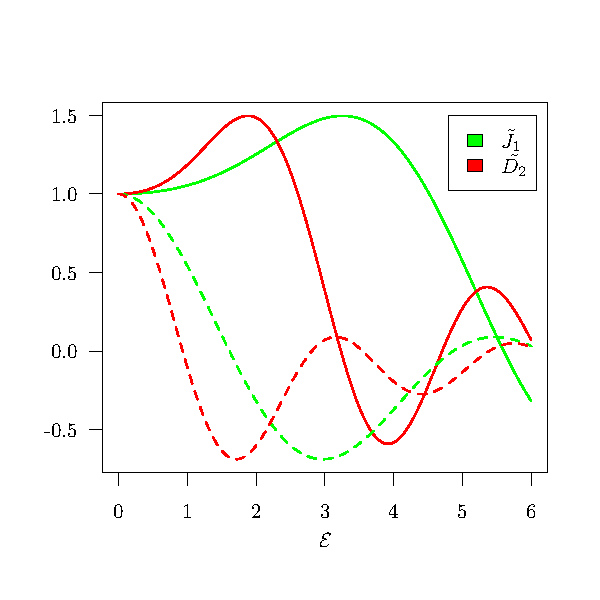
\includegraphics[width=1\linewidth]{Figures/NNvsNNN1.pdf}
  \caption{$\frac{J_{1}}{J_{1}^0}$ and $\frac{D_{2,ij}}{D_{2,ij}^0}$ are plotted as function of $\mathcal{E}$. Similar results are obtained in \cite{Mentink2015} for $J_{1}$. Solid lines are for $\omega = 4$ and dashed lines are for $\omega = 14$.}
  \label{Fig3.1:NNvsNNN}
\end{subfigure}%
\hspace*{\fill}
\begin{subfigure}{.45\textwidth}
  %\centering
  \includegraphics[width=1\linewidth]{Figures/ratio.pdf}
  \caption{$\frac{J_{1}}{D_{2,ij}}$ is plotted as function of $\mathcal{E}$, it diverges every time $D_{2,ij}$ changes sign. Solid lines are for $\omega = 4$ and dashed lines are for $\omega = 14$.}
  \label{Fig3.1:ratio}
\end{subfigure}
\label{Fig3.1}
\end{figure}

\begin{figure}
\centering
  \includegraphics[width=0.5\linewidth]{Figures/theta.pdf}
  \caption{The spin wave density NN angle $\theta$ as a function of $\mathcal{E}$. The field modifies the ratio $\frac{J_{1}}{D_{2,ij}}$ thus modifying the wave vector. Solid lines are for $\omega = 4$ and dashed lines are for $\omega = 14$.}
\label{Fig3.2}
\end{figure}

\end{subsection}

\begin{subsection}{Two dimensional systems}
 
In a honeycomb lattice described by the effective spin model \ref{MKMHeff} the usual approach is to write:

\begin{align}
\bs{S}_1(\bs{r}) &= S\left( \cos(\bs{Q}\bs{r}), \sin(\bs{Q}\bs{r}), 0 \right) \\
\bs{S}_2(\bs{r}) &= -S\left( \cos(\bs{Q}\bs{r} + \theta), \sin(\bs{Q}\bs{r} + \theta), 0 \right)
\end{align}

The $1, 2$ subindex stands for the sublattice. The $\hat{e}_z$ component vanishes in order to minimize the contribution of the pseudodipolar interaction. Let $Q_a = \bs{Q}\hat{\bs{a}}$ and $Q_b = \bs{Q}\hat{\bs{b}}$, where $\hat{\bs{a}}$ and $\hat{\bs{b}}$ are the primitive cell vectors. Then, the classical energy per spin is given by:

\begin{align}
\frac{E}{NS^2} &= -\frac{J_1}{2}\left( \cos(\theta) + \cos(\theta - Q_a - Q_b) + \cos(\theta - Q_b) \right) + \nonumber \\
&+ (J_2-\Gamma) \left( \cos(Q_a) + \cos(Q_b) + \cos(Q_a+Q_b) \right)+ \nonumber \\
&+D_2\left( \sin(Q_a) + \sin(Q_b) + \sin(Q_a+Q_b) \right)
\end{align}

Notice that when the spins are constrained in the $\hat{e}_x, \hat{e}_y$ plane, the anisotropic interaction $\bs{S}_i\bs{\Gamma}_{ij}\bs{S}_j$ becomes a ferromagnetic interaction. The minimization of this energy will lead to an involved phase diagram in the $J_1, J_2, D_2, \Gamma_2$ space (or equivalently, in the $t_1, t_2, \Delta$ space). We will not attempt to describe this phase diagram. However, as we have shown in the one dimensional case, by modulating the laser amplitude we can control the ratio between the NN and NNN coupling factors, and thus the parameters $\bs{Q}$ and $\theta$ of the system state.

\end{subsection}

\end{section}


\begin{subappendices}
\begin{section}{Peierls Substitution}
\label{AP3A}

In first quantization we can introduce a vector potential $\bs{A}(\bs{r},t)$ by changing the Hamiltonian of the lattice \ref{LaticeHam} to:

\begin{equation}
\label{HamEMF}
  \hat{H}'(\bs{r}) = \frac{(\bs{p}-e\bs{A})^2}{2m} +U(\bs{r})
\end{equation}

Now the Bloch functions defined for \ref{LaticeHam} will not be eigenfunctions of this Hamiltonian. We define a new set of Wannier functions in terms of those defined in \ref{Wannier2}, and obtain the new Bloch functions. 

\begin{align}
\psi'_{\bs{R}}(\bs{r}) &= e^{i\frac{e}{\hbar}\int_{\bs{R}}^{\bs{r}} d\bs{r}'\bs{A}(\bs{r}',t)} \psi_{\bs{R}}(\bs{r}) \\
\phi'_{\bs{k}}(\textbf{r}) &= \frac{1}{\sqrt{M}}\sum_{\bs{R}} e^{-i\bs{k}\bs{R}}\psi'_{\bs{R}}(\bs{r}) = \frac{1}{\sqrt{M}}\sum_{\bs{R}} e^{-i\bs{k}\bs{R}} e^{i\frac{e}{\hbar}\int_{\bs{R}}^{\bs{r}} d\bs{r}'\bs{A}(\bs{r}',t)} \psi_{\bs{R}}(\bs{r})
\end{align}

Where we omitted the band number. The action of the new Hamiltonian is greatly simplified:

\begin{align*}
\hat{H}'(\bs{r}) \psi'_{\bs{R}} (\bs{r}) &= \left[ \frac{(\bs{p}-e\bs{A})^2}{2m} +U(\bs{r}) \right] e^{i\frac{e}{\hbar}\int_{\bs{R}}^{\bs{r}} d\bs{r}'\bs{A}(\bs{r}',t)} \psi_{\bs{R}}(\bs{r}) = \\
&=e^{i\frac{e}{\hbar}\int_{\bs{R}}^{\bs{r}} d\bs{r}'\bs{A}(\bs{r}',t)} \left[ \frac{(\bs{p} - i\hbar \bs{\nabla_r}(i\frac{e}{\hbar}\int_{\bs{R}}^{\bs{r}} d\bs{r}'\bs{A}(\bs{r}',t)) -e\bs{A})^2}{2m} +U(\bs{r}) \right] = \\
&= e^{i\frac{e}{\hbar}\int_{\bs{R}}^{\bs{r}} d\bs{r}'\bs{A}(\bs{r}',t)} \left[ \frac{\bs{p}^2}{2m} + U(\bs{r}) \right] \psi_{\bs{R}}(\bs{r}) = e^{i\frac{e}{\hbar}\int_{\bs{R}}^{\bs{r}} d\bs{r}'\bs{A}(\bs{r}',t)} \hat{H}(\bs{r}) \psi_{\bs{R}}(\bs{r})
\end{align*}

And so, the matrix elements as in the case without field except for a phase:

\begin{equation}
\label{PeierlsMtxElem}
t_{ij}(t) = \bra{\psi'_{\bs{R_i}}} \hat{H}'(\bs{r}) \ket{\psi'_{\bs{R_j}}} = e^{i\frac{e}{\hbar}\int_{\bs{R}_j}^{\bs{R}_i} d\bs{r}'\bs{A}(\bs{r}',t)} \bra{\psi_{\bs{R_i}}} \hat{H}(\bs{r}) \ket{\psi_{\bs{R_j}}}
\end{equation}

When the field can be approximated as constant along the lattice we have: $e^{i\frac{e}{\hbar}\int_{\bs{R}_j}^{\bs{R}_i} d\bs{r}'\bs{A}(\bs{r}',t)} = e^{i\frac{e}{\hbar} (\bs{R}_i-\bs{R}_j) \bs{A}(t)}$.

Notice that this substitution also applies if we add a Rashba Spin-Orbit interaction term to \ref{HamEMF}, i.e., if $\hat{H}'(\bs{r}) = \frac{(\bs{p}-e\bs{A})^2}{2m} +U(\bs{r}) + \alpha_R \hat{z}(\hat{\bs{\sigma}} \times (\bs{p}-e\bs{A}))$, then

\begin{align*}
  \alpha_R \hat{z}(\hat{\bs{\sigma}} \times (\bs{p}-e\bs{A})) \psi'_{\bs{R}} &= \alpha_R(\hat{\sigma_x}(\hat{p}_y-e\bs{A}) - \hat{\sigma_y}(\hat{p}_x-e\bs{A})) e^{i\frac{e}{\hbar}\int_{\bs{R}}^{\bs{r}}d\bs{r}'\bs{A}(\bs{r}',t)} \psi_{\bs{R}} = \\
  &= e^{i\frac{e}{\hbar}\int_{\bs{R}}^{\bs{r}}d\bs{r}'\bs{A}(\bs{r}',t)} \alpha_R \hat{z}\hat{\bs{\sigma}} \times \bs{p} \psi_{\bs{R}}
\end{align*}

Therefore relation \ref{PeierlsMtxElem} still holds.

\end{section}

\begin{section}{Identities}
\label{AP3B}
Let $Z(t)$ be an operator dependent on the parameter $t$. Then:

\begin{align*}
d_t e^{Z} &= d_t \sum_{n=0}^\infty \frac{1}{n!} Z^n = \sum_{n=0}^\infty \sum_{m=0}^{n-1} \frac{1}{n!} Z^m \frac{\partial Z}{\partial t} Z^{n-m-1} = \\
&= \sum_{m=0}^\infty \sum_{p=0}^\infty \frac{1}{(m+p+1)!}Z^m \frac{\partial Z}{\partial t} Z^p = \sum_{m=0}^\infty \sum_{p=0}^\infty \frac{m!p!}{(m+p+1)!} \frac{Z^m}{m!} \frac{\partial Z}{\partial t} \frac{Z^p}{p!} =\\
&= \sum_{m=0}^\infty \sum_{p=0}^\infty \int_0^1 dx x^m (1-x)^p \frac{Z^m}{m!} \frac{\partial Z}{\partial t} \frac{Z^p}{p!} = \int_0^1 dx e^{Zx} \frac{\partial Z}{\partial t} e^{Z(1-x)} = \\
&= \int_0^1 dx \sum_{n=0}^\infty \frac{1}{n!} \left[xZ, \dots, \left[xZ, \frac{\partial Z}{\partial t}\right] \dots \right] e^Z = \sum_{n=0}^\infty \frac{1}{(n+1)!} \left[Z, \dots, \left[Z, \frac{\partial Z}{\partial t}\right] \dots \right] e^Z
\end{align*}

Where we used the Beta function $\int_0^1 dx x^m (1-x)^p = \frac{m!p!}{(m+p+1)!}$ and we also used the Baker–Campbell–Hausdorff expansion for $e^{xZ}\frac{\partial Z}{\partial t}e^{-xZ}$ and $\int_0^1 x^n = \frac{1}{n+1}$. Therefore we proved:

\begin{equation}
\label{SneidersID}
d_t e^{Z} = \sum_{n=0}^\infty \frac{1}{(n+1)!} \left[Z, \dots, \left[Z, \frac{\partial Z}{\partial t}\right] \dots \right] e^Z = \sum_{n=0}^\infty \frac{1}{(n+1)!} \text{ad}_Z ^n \left(\frac{\partial Z}{\partial t}\right) e^Z
\end{equation}

Where $\text{ad}_A(B) = [A,B]$.

\end{section}

\end{subappendices}







